% ----------------------------------------------------------
% Teoria
% ----------------------------------------------------------
\chapter{Teoria}
\label{chap:teoria}

O trabalho desenvolvido nesta tese tem como base métodos de
solução numérica de equações diferenciais parciais. Não é objetivo,
tamanha seria a ousadia, discorrer sobre as bases teóricas da neutrônica ou
da termo-hidráulica. Neste capítulo, são, portanto, apresentados, de forma simplificada,
o funcionamento dos cálculos de mecânica dos fluidos computacional (CFD) e dos
cálculos neutrônicos, baseados aproximação por difusão da equação de transporte
de nêutrons.

%\begin{figure}[htb]
%  \caption{Teoria: o sistema acoplado.}
%  \centering\includegraphics[scale=0.7]{figuras/teoria1.png}
%  \label{metodoetapas}
%  \legend{Fonte: autor}
%\end{figure}

% **********************************************
\section{Termo-hidráulica}
\label{sec:th}

A Termo-hidráulica é a área de estudo dos de transferência
de calor e massa, processos fluido-mecânicos com transporte de energia e
massa em sistemas nucleares. Os principais fenômenos estudados incluem condução,
convecção, transferência de calor por radiação, mudanças de fase e escoamentos
monofásicos e multifásicos.

A análise termo-hidráulica de sistemas de conversão de energia envolve a solução
das equações de transporte de massa, momento e energia \cite{Todreas2012}. Nesta
tese, a análise deste tipo de sistema é feita utilizando-se o a mecânica
de fluidos computacional (CFD). O CFD é, grosso modo, uma forma de se resolver
problemas físicos complexos pelo uso de métodos numéricos em sistemas
computacionais. Tais métodos numéricos, funcionam descrevendo equações diferenciais
válidas em domínios contínuos em sistemas de equações algébricas, de modo que
sejam resolvidos numericamente. Para transformar o sistema contínuo num sistema
discreto, o domínio contínuo é discretizado em um conjunto de subdomínios menores
e conectados que formam uma malha de pequenos elementos, chamados
alternativamente de volumes ou células \cite{dosSantos2012}. 
A partir deste domínio discreto, Figura \ref{fig:dom}, a solução numérica é ser obtida.

\begin{figure}[htb]
  \caption[Domínio contínuo e discretizado.]{Domínio contínuo (à esquerda) e discretizado (à direita).}
  \centering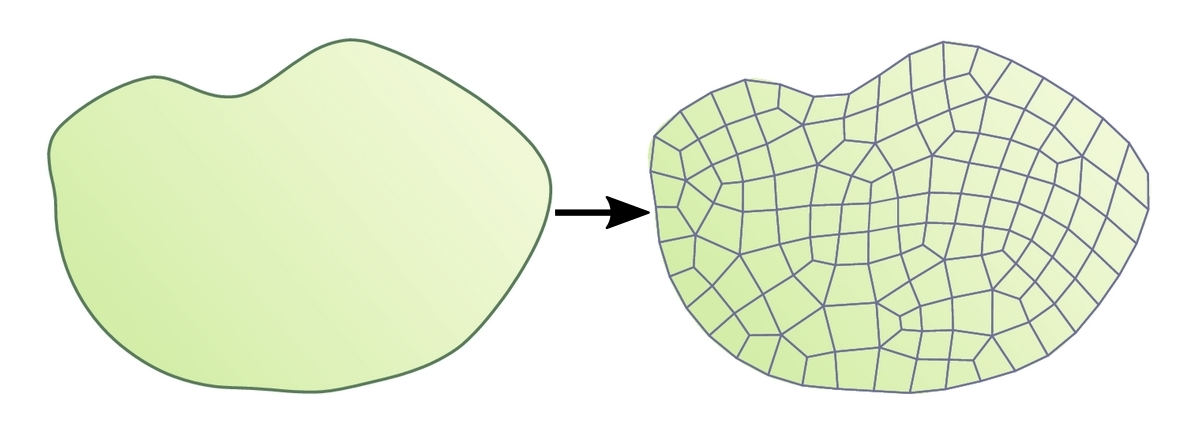
\includegraphics[scale=1.3]{figuras/dom.png}
  \label{fig:dom}
  \legend{Fonte: \cite{Theler2013b}}
\end{figure}

A análise por CFD envolve, geralmente, quatro etapas distintas:

\begin{itemize}
\item Geração da malha (ou preprocessamento): A partir da geometria do sistema, que equivale ao
  domínio contínuo, é necessário gerar uma malha. Essa malha pode ser refinada
  em pontos estratégicos, ser estruturada ou não-estruturada e possuir elementos
  de diferentes formatos. A malha utilizada na solução de um problema tem impacto
  direto no tempo de simulação, na qualidade da solução e até mesmo no alcance
  da solução. Em um projeto de CFD, aproximadamente 50\% do tempo é dedicado a geração
  da geometria e da malha \cite{Versteeg2007}.
\item Modelagem matemática: Equivale a definir, com base no conhecimento
  físico do problema, as hipóteses válidas, eventuais simplificações e
  seus impactos na solução final. A partir das definições, é necessário
  descrever as condições iniciais e de contorno de problema, as propriedades
  termo-físicas, químicas, fenômenos modelados e quaisquer outras características
  necessárias à solução do problema.
\item Solução: Nesta etapa são resolvidos os sistemas lineares obtidos pela
  discretização do domínio. Um dos métodos de discretização mais utilizados
  em problemas envolvendo comportamento de fluidos é o de volumes finitos. Além dos
  métodos de discretização, há diversos métodos para a solução dos sistemas
  lineares resultantes da discretização, com melhor ou pior desempenho de
  acordo com características do sistema linear a ser resolvido \cite{Barrett1994}.
\item Análise dos resultados (ou pós-processamento): Após a finalização
  com sucesso da simulação, os usuário deve tratar a grande quantidade de
  dados obtidos. Esta etapa consiste em extrair os resultados qualitativos
  e quantitativos, através do uso de ferramentas de visualização, estatística,
  matemáticas dentre outras \cite{Maric2014}.
\end{itemize}

Nos cálculos por CFD são resolvidas as equações fundamentais de transporte de massa (Equação \ref{eq:massa}),
momento (Equação \ref{eq:momento}) e energia (Equação \ref{eq:energia}), apresentadas abaixo em notação tensorial compacta \cite{dosSantos2012}.

\begin{equation}
%  \centering
  \label{eq:massa}
  \frac{\partial \rho}{\partial t}+\frac{\partial}{\partial x_j}(\rho u_j)=0
\end{equation}

\begin{equation}
%  \centering
  \label{eq:momento}
  \frac{\partial \rho u_i}{\partial t}+\frac{\partial}{\partial x_j}(\rho u_i u_j)=
  -\frac{\partial p}{\partial x_i} + \frac{\partial}{\partial x_j}\bigg[ \mu \bigg( \frac{\partial u_i}{\partial x_j} + \frac{\partial u_j}{\partial x_i}\bigg)\bigg]+S_{Mi}
\end{equation}

\begin{equation}
%  \centering
  \label{eq:energia}
  \frac{\partial \rho h_{tot}}{\partial t}-\frac{\partial \rho}{\partial t}+\frac{\partial}{\partial x_j}(\rho u_i h_{tot})=
  \frac{\partial p}{\partial x_j}\bigg( \lambda \frac{\partial T}{\partial x_i}\bigg) + \frac{\partial}{\partial x_j}\bigg[ u_i\mu \bigg( \frac{\partial u_i}{\partial x_j} + \frac{\partial u_j}{\partial x_i}\bigg)\bigg]+S_{E}
\end{equation}

Sendo $h_{tot} = h_{(T,p)} + \frac{u_i^{2}}{2}$ a entalpia total e $S_{Mi}$ e $S_E$, respectivamente, os termos
fonte das equações de momento e energia.

De acordo com a natureza do processo a ser simulado, alguns termos podem ser omitidos. Para o
caso de um cálculo estacionário, os termos relacionados à variações no tempo são
considerados nulos. Geralmente, tais simplificações levam consequentemente a
simplificações nos cálculos.

%Nesta seção serão apresentadas
%as equações utilizadas na modelagem de um sistema termo-hidráulico monofásico e
%estacionário.

% **********************************************
%\subsection{Equações governantes}
%\label{subsec:eq}


% **********************************************
%\subsubsection{Fluidos}
%\label{ssubsec:fluid}

% **********************************************
%\subsection{Turbulência}
%\label{subsec:turb}

%A modelagem da turbulência 
% **********************************************
%\subsection{Modelo termo-hidráulico discretizado}
%\label{subsec:modeloth}


% **********************************************
%\subsubsection{Sólidos}
%\label{ssubsec:solid}

% **********************************************
\section{Neutrônica}
\label{sec:neutronica}

Neutrônica pode ser definida como o estudo do movimento e interações dos nêutrons
com a matéria. O conhecimento de neutrônica é fundamental para determinar o
comportamento de um reator nuclear ou outros elementos que utilizem nêutrons
em feixes. A neutrônica é, em última instância, o estudo do transporte de nêutrons.

A probabilidade de interação entre um nêutron incidente e um núcleo alvo é caracterizada
pela seção de choque microscópica (unidade \textit{barn}, símbolo $\sigma$ e
equivalente a $10^{-24} cm^2$), que depende do núcleo alvo, do tipo de interação e da
energia do nêutron incidente. Essa dependência pode ser complicada devido a diversos fatores,
como a ordem de grandeza das energias envolvidas, levando a variações súbitas nas probabilidades
de interação. Estas variações são chamadas ressonâncias. A seção de choque macroscópica nada mais
é do que a seção de choque microscópica multiplicada pela densidade nuclear. Ela dá as probabilidades
médias de reação entre nêutrons de determinada energia com o material presente considerando a massa
do material. Sua unidade é dada em $cm^{-1}$.

%No escopo desta tese, é suficiente afirmar que as seções de choque são elementos fundamentais
%na descrição e, portanto, no cálculo neutrônico. 

% **********************************************
\subsection{Dados nucleares}
\label{subsec:dn}

% Do Hebért
A colisão entre um nêutron e um núcleo pode produzir reações nucleares de diferentes
tipos. Em um caso simples, o nêutron é simplesmente desviado, numa colisão elástica.
Em outros casos, esta interação pode produzir um núcleo composto, quando o nêutron é
absorvido pelo núcleo alvo. Neste caso, a energia do nêutron incidente é transmita para
o núcleo alvo que se torna instável. As formas de liberação dessa energia podem ser desde
a liberação de raios gama até a fissão deste núcleo.

O conceito de seção de choque \cite{Hebert2009} é usado para descrever a probabilidade
de cada tipo de reação nuclear e é baseado em propriedades fundamentais que caracterizam
as interações nucleares com os nêutrons.

A seção de choque microscópica ($\sigma_x$) é um fator de proporcionalidade numa relação entre
a taxa de reações numa determinada superfície e o número de nêutrons vezes a velocidade
relativa dos nêutrons em relação ao alvo e a densidade de nêutrons no feixe incidente.
Sua unidade é a unidade de superfície, data usualmente em $barns$ ($b=10^{-24}cm^2$).

A seção de choque macroscópica é definida a partir da seção de choque microscópica ($\Sigma_x$)
multiplicada pela densidade do material (que pode ou não ser composto por diferentes elementos ou
isótopos). É dada em $cm^{-1}$ e representa a chance efetiva de interação de um nêutron incidente
com todos os núcleos em um dado volume.

Fundamental para os cálculos neutrônicos, a obtenção de seções de choque representativas para
o sistema que se pretende calcular é usualmente feita a partir de bibliotecas de seções de choques
contínuas. Estas bibliotecas são utilizadas como entrada para códigos capazes de processar
as seções de choques contínuas, como o WIMS \cite{Halsall1986},
em bibliotecas de seções de choque isotópicas colapsadas em grupos.
Estas seções de choque processadas são então utilizadas tanto em cálculos por métodos
estocásticos quanto determinísticos.


% **********************************************
\subsection{Métodos estocásticos}
\label{subsec:mc}

Uma das formas de se modelar a interação de partículas, no presente caso nêutrons,
com a matéria, que por sua vez pode ser um fluido, gás ou sólido, é através de
métodos estocásticos (ou probabilísticos). As técnicas baseadas em números
aleatórios são chamadas de Monte Carlo devido ao famoso cassino com este nome
localizado em Mônaco.

As técnicas de Monte Carlo, ou especificamente chamado método de Monte Carlo
nas ciências nucleares, se baseiam na probabilidade de que determinados eventos,
quanto testados um número suficiente de vezes, possam ser representados
com acurácia por probabilidades

Na neutrônica, uma das formas de se representar o transporte
e colisões entre nêutrons é através do
uso do método de Monte Carlo \cite{Hutchinson2015}.

%Na Figura \ref{fig:random_walk}
%são mostradas algumas interações possíveis de um nêutron, desde seu surgimento
%até sua absorção.

%\begin{figure}[htb]
%  \caption{Exemplo de interações de um nêutron com a matéria.}
%  \centering\includegraphics[scale=0.5]{figuras/random_walk.png}
%  \label{fig:random_walk}
%  \legend{Fonte: autor}
%\end{figure}

O objetivo principal das simulações por Monte Carlo é, geralmente, determinar
o valor médio de algum parâmetro relativo ao comportamento das partículas simuladas, como o fluxo de
nêutrons em função de sua posição, por exemplo. Cabe lembrar que, por depender
de um grande número de eventos para ser estatisticamente válida, uma única
simulação por Monte Carlo pode extremamente custosa do ponto de vista computacional.
Ainda assim, o método é cada vez mais utilizado e, com o aumento de poder
computacional atual, mais viável para problemas complexos.

Uma breve introdução às técnicas de Monte Carlo, com ênfase no uso para
transporte de radiação e em nível de estudantes, pode ser encontrado
no livro de Hutchinson \cite{Hutchinson2015}.

% Falar de random walk
% Colisão e o que acontece
% Iteração com outras partículas
% Tracking e talling
% Incerteza

% **********************************************
\subsection{Métodos determinísticos: a aproximação por difusão}
\label{subsec:det}

A assim chamada aproximação por difusão é usualmente utilizada para cálculos
do fluxo neutrônico no núcleo de reatores, normalmente utilizando a teoria
de difusão para poucos grupos de nêutrons \cite{Hebert2009}.

A equação de difusão é obtida pela substituição da Lei de Fick na equação de
transporte integrada em todo o volume de cálculo, além de assumir
diversas simplificações \cite{Theler2013b}. A Lei de Fick funciona como
uma relação heurística entre entre o fluxo e a corrente de nêutrons.
Esta relação, entretanto, impõe algumas limitações nos problemas a serem
resolvidos. A Lei de Fick não é válida próxima a regiões
de descontinuidade, na proximidade de pontos de fuga ou termos-fonte, quanto
a anisotropia é suficientemente alta (quando a seção de choque
de absorção e da mesma ordem de grandeza da seção de choque total), em
meios altamente absorvedores, na proximidade de interfaces e quando há variação
rápida do fluxo (não é o caso em casos estacionários).
Algumas destas limitações, porém, podem ser corrigidas
em vários casos. A equação da difusão consiste
num conjunto de equações diferenciais parciais de segunda ordem resolvidas
em coordenadas espaciais.

A equação de difusão para multi-grupos é dada pela equação \ref{eq:dif} \cite{Demaziere2014}:

\begin{equation}
  \label{eq:dif}
  %    \begin{split}
  -\nabla.[D_g(\mathbf{r})]\nabla \phi_g(\mathbf{r})+ \Sigma_{(T,g)}(\mathbf{r})\phi_g(\mathbf{r}) =
  \sum_{g'=1}^{G} \Sigma_{s0,g'\rightarrow g}(\mathbf{r})\phi_{g'}(\mathbf{r}) +
  \frac{\chi_g}{k}\sum_{g'=1}^{G}\nu_{g'}\Sigma_{f,g'}(\mathbf{r})\phi_{g'}(\mathbf{r})
  %\end{split}
\end{equation}

% Tabelar os termos

A equação de difusão pode ser resolvida analiticamente para casos simples, em geral em
casos didáticos, ou utilizando técnicas padrão de análise numérica, como o método de
elementos finitos ou volumes finitos.

Apesar de aparentemente grosseira devido às simplificações para sua obtenção, a equação
de difusão dá resultados próximos aos obtidos por métodos mais elaborados \cite{Theler2013b}.

É importante ressaltar que a Equação \ref{eq:dif} é um problema de \textit{autovalor}, cuja
solução existe para distintos autovalores $k$. O maior autovalor absoluto corresponde à
solução fundamental do problema de autovalor e é igual ao fator de multiplicação
efetivo ($k_{eff}$) do reator. Apenas a solução fundamental tem significado físico.

A compacta apresentação dada neste texto para as equações de Navier-Stokes e para a
equação de difusão visa apenas introduzir
as bases fundamentais dos problemas que são resolvidos pelos sistemas acoplados nesta tese.

% **********************************************
%\subsubsection{Equação de Transporte}
%\label{ssubsec:transp}

% **********************************************
% \subsubsection{Aproximação por Difusão}
% \label{ssubsec:difusao}

% **********************************************
%\subsection{Modelo neutrônico discretizado}
%\label{subsec:modelon}

